\section{Wave Energy Resources of the United States}
\label{sec:results}

We estimate the total wave energy resource of the U.S. to be 3300 TWh/yr, and the near-shore resource to be 1900 TWh/yr (Table~\ref{table:totals}). 
These values are, respectively, 25\% higher than and 39\% lower than the EPRI 2011 wave resource assessment \citep[][]{EPRIwaveresource2011}. 
Because the integration contour used in EPRI 2011 is between the EEZ and near-shore boundaries we use here, these results are qualitatively consistent with EPRI's estimate. 
At the same time, these results are more accurate due to improvements in the methodology and underlying models. Furthermore, the difference between the full-EEZ and near-shore results emphasize the importance of being clear and consistent when choosing the boundary where the wave resource is estimated.

Wave energy has a consistent seasonal cycle across all regions: it is a late-fall and winter dominated resource (Figure \ref{fig:annual-cycle}), with a peak in December or January and a minimum in summer. This has the potential to compliment solar energy generation projects. 

The inter-annual variability of the resource is generally proportional to the resource amplitude: low variability in summer and high-variability in winter. During energetic boreal winter months (December, January, February), the monthly-averaged resource can vary by more than 50\%, but in general the inter-annual variability is less than 30\% of the month's mean. This suggests that during these energetic winter months wave energy projects should be expected to deliver the total-mean (average across years and months) at a minimum with the potential to provide up to three times the value of the total mean wave resource.

\subsection{The U.S. West Coast}

The west coast is a promising region for wave energy because it possesses a large total resource (510 TWh/yr) and has the coastal population density to make use of it. The inner-shelf resource (410~TWh/yr) is equal to $\sim40$\% of the electricity consumption of California, Oregon, and Washington (2018 total: 943 TWh/yr), which suggests there is sufficient resource to play a sizable role in the region's energy profile in the foreseeable future \citep{energyinformationadministrationStateEnergyConsumption2020}. The resource along the northern half of the west coast — Oregon, Washington, and Northern California — is particularly energetic: the annual-average wave energy flux exceeds 40 kW/m in several places.

This resource is composed primarily of long-period waves — 90\% of the resource is contained between 6.5 and 19 seconds (Figure \ref{fig:remote-freq}) — which carry more energy per-unit of wave amplitude. These waves arrive at the shoreline from throughout the Pacific basin \citep{perezESTELAMethodEvaluating2014}. The PacWave test site, offshore of central Oregon, has been created to be the first U.S. "grid-connected full-scale test facility", is critical to testing wave technologies and demonstrating that they can perform efficiently and reliably in this world-class fully-energetic environment where winter storms regularly deliver waves with more than 8 meters in amplitude \citep[e.g.][]{allan_climate_2006}.


\subsection{The U.S. East Coast}

The east coast also possesses a sizable wave energy resource (290 TWh/yr), but it is composed primarily of the local resource (180 TWh/yr). This is because mid-latitude westerly winds tend to generate wave energy that propagates eastward and builds to a sizable resource across the broad fetch of the U.S. EEZ. Relatively less wave energy from the open Atlantic propagates onshore toward the U.S. eastern coastline, which contrasts with the West Coast that receives significant energy from the trans-Pacific swells. The remote resource, therefore, is relatively modest (110 TWh/yr at the EEZ, and 90 TWh/yr on the inner-shelf). Because this resource is dominated by waves that are generated locally, the waves tend to be much shorter-period (90\% of the energy is between 6 and 15 seconds, Figure \ref{fig:remote-freq}).

The offshore directed winds cause the most energetic wave resource to be located near the edge of the EEZ offshore of New England (Figure~\ref{fig:map-total}). Note here that the omni-directional wave power shows the combined effect of local and remote resource. The east coast inner-shelf resource is somewhat smaller than the EEZ remote resource because a fraction of energy in these westward-propagating remote waves are dissipated by white-capping from the westerly winds.

While the East Coast wave resource is modest in comparison to the West Coast, the potential for wave energy cannot be neglected. As wave technologies continues to mature and if the cost of the technology is low enough, sites and regions previously considered uneconomical may prove to be attractive, especially in markets where energy prices are already high and alternate renewable sources are limited or constrained. 

\subsection{Hawaii}

Hawaii also possesses a large resource (380 TWh/yr) composed primarily of waves propagating southward from the North Pacific. The local resource is relatively small (10 TWh/yr), due primarily to the fact that the sea-state in this region is -- in the long-average perspective of regional resource assessment -- approximately `steady-state' because the wind input and dissipation are nearly in balance. The inner-shelf Hawaiian resource (120 TWh/yr) is smaller than the EEZ remote resource because the 10 nautical-mile boundary is a much ``smaller net'' in comparison to the full EEZ.

Hawaii is a particularly interesting case because the resource is large compared to the State's electricity consumption (26 TWh/yr), and because energy-prices are high. Wave energy may be particularly valued in Hawaii where space is limited for land-based renewable alternatives; and the tourist economy may especially value WECs with limited surface expression. Together, these factors make Hawaii a likely early-market for wave energy technology. The Navy's Wave Energy Test Site on the north shore of Oahu, is supporting the development and demonstration of technologies for meeting the potential demand \citep{crossEarlyResearchEfforts2015}.

The Hawaiian resource is bi-modal with peaks at 13 and 9 seconds. This ``double-peak'' is primarily a seasonal effect where longer-period waves (12-14 seconds) are more prevalent in January and February, while shorter-period waves (8-10 seconds) arrive in March and April \citep[][]{stopa2013wave}. 

\subsection{Alaska}

Nearly two-thirds of the nation's wave energy resource is in Alaska (2000 TWh/yr). However, the majority of this resource is `stranded' very far from markets large enough to utilize more than a few MW of power. Still, if the cost of large-scale energy storage technologies becomes sufficiently economical (e.g., renewable fuels, batteries, etc.), or if energy-intensive industrial activity were sited in this region, this wave resource could become valuable. In the shorter-term, the villages along Alaska's coastline -- where energy prices are very high -- represent an opportunity to demonstrate commercial viability before scaling the technology up \citep{alaskaenergyauthority2019PowerCost2020}. Or this energy could be used in-place for Blue Economy applications such as charging batteries on vessels or for scientific instruments during long transits or exploration. 

\subsection{Gulf of Mexico, Puerto Rico, and U.S. Virgin Islands}

The Gulf of Mexico's wave resource is small compared to the rest of the regions, composed almost exclusively of locally-generated, short-period waves. The wide shelf in this region also has the effect of damping some of the wave energy. The presence of hurricanes in this region confounds the challenge of developing wave energy projects because devices would need to be designed to survive the extreme conditions that come with hurricanes. The same basic conclusions can also be drawn for Puerto Rico and the U.S. Virgin Islands. Throughout the Gulf and these islands there may be niche applications, or specific sites, where wave energy can be utilized. But it seems unlikely that utility-scale wave power will contribute significantly to the power needs.


%\begin{table}[ht]
%  \centering
%  \begin{tabular}{|c|c|c|c|c|c|}
%    %\cline{2-7}
%    %%\multirow{1}{*}{Region}
%    %\multicolumn{1}{c|}{} & {\it EPRI 2011} & \multicolumn{5}{c|}{New} \\
%    \hline
%    Region & Inner-Shelf & Remote & \multicolumn{2}{c|}{Local} & Total \\
%    & & & Natural & {\it Potential} & \\
%    \hline
%    Alaska & 1190 & 1040 & 990 & {\it 1510} & 2030 {\it – 2550} \\
%    West Coast & 410 & 420 & 90 & {\it 210} & 510 {\it – 630} \\
%    Hawaii & 120 & 370 & 10 & {\it 100} & 380 {\it – 470} \\
%    East Coast & 90 & 110 & 180 & {\it 230} & 290 {\it – 340} \\
%    Gulf of Mexico & 20 & 13 & 56 & {\it 57} & 69 {\it – 70} \\
%    P.R. \& U.S.V.I. & 20 & 6 & 11 & {\it 27} & 17 {\it – 33} \\
%    \hline \hline
%U.S. TOTAL & 1850 & 1960 & 1340 & 2130 & 3300 {\it – 4090} \\
%\hline
%  \end{tabular}
%  \caption{Wave resource assessment results by region and totaled for the entire U.S. (all values in TWh/yr). The range in %the "Total" column indicates the sum of Remote + Local (lower value) and Remote + Potential (higher value, in italics).
%  \noteSelf{Do we need to be more careful w/ significant digits here?}
%  }
%  \label{table:totals}
%\end{table}



\begin{table}[ht]
  \centering
  \begin{tabular}{|c|c|c|c|c|}
    %\cline{2-7}
    %%\multirow{1}{*}{Region}
    %\multicolumn{1}{c|}{} & {\it EPRI 2011} & \multicolumn{5}{c|}{New} \\
    \hline
    Region & Inner-Shelf & Remote & Total & Potential \\
    \hline
    Alaska & 1200 & 1000 & 2000 & +520 \\
    West Coast & 410 & 420 & 510 & +120 \\
    Hawaii & 120 & 370 & 380 & +90 \\
    East Coast & 90 & 110 & 290 & +50 \\
    Gulf of Mexico & 20 & 13 & 69 & +1 \\
    P.R. \& U.S.V.I. & 20 & 6 & 17 & +16 \\
    \hline \hline
    U.S. Total & 1900 & 2000 & 3300 & +790 \\
    \hline
  \end{tabular}
  \caption{Theoretical wave resource results by region and totaled for the entire U.S. (all values in TWh/yr). The inner-shelf resource is the remote resource 10-nautical-miles from shore. The total is the sum of the local and remote resource, and the potential is how much additional energy is available if the entirety of the remote resource is removed at the EEZ boundary. All values are reported to two significant figures, therefore totals may not equal sum of regional values.
  }
  \label{table:totals}
\end{table}

\begin{figure}[ht]
  \centering
  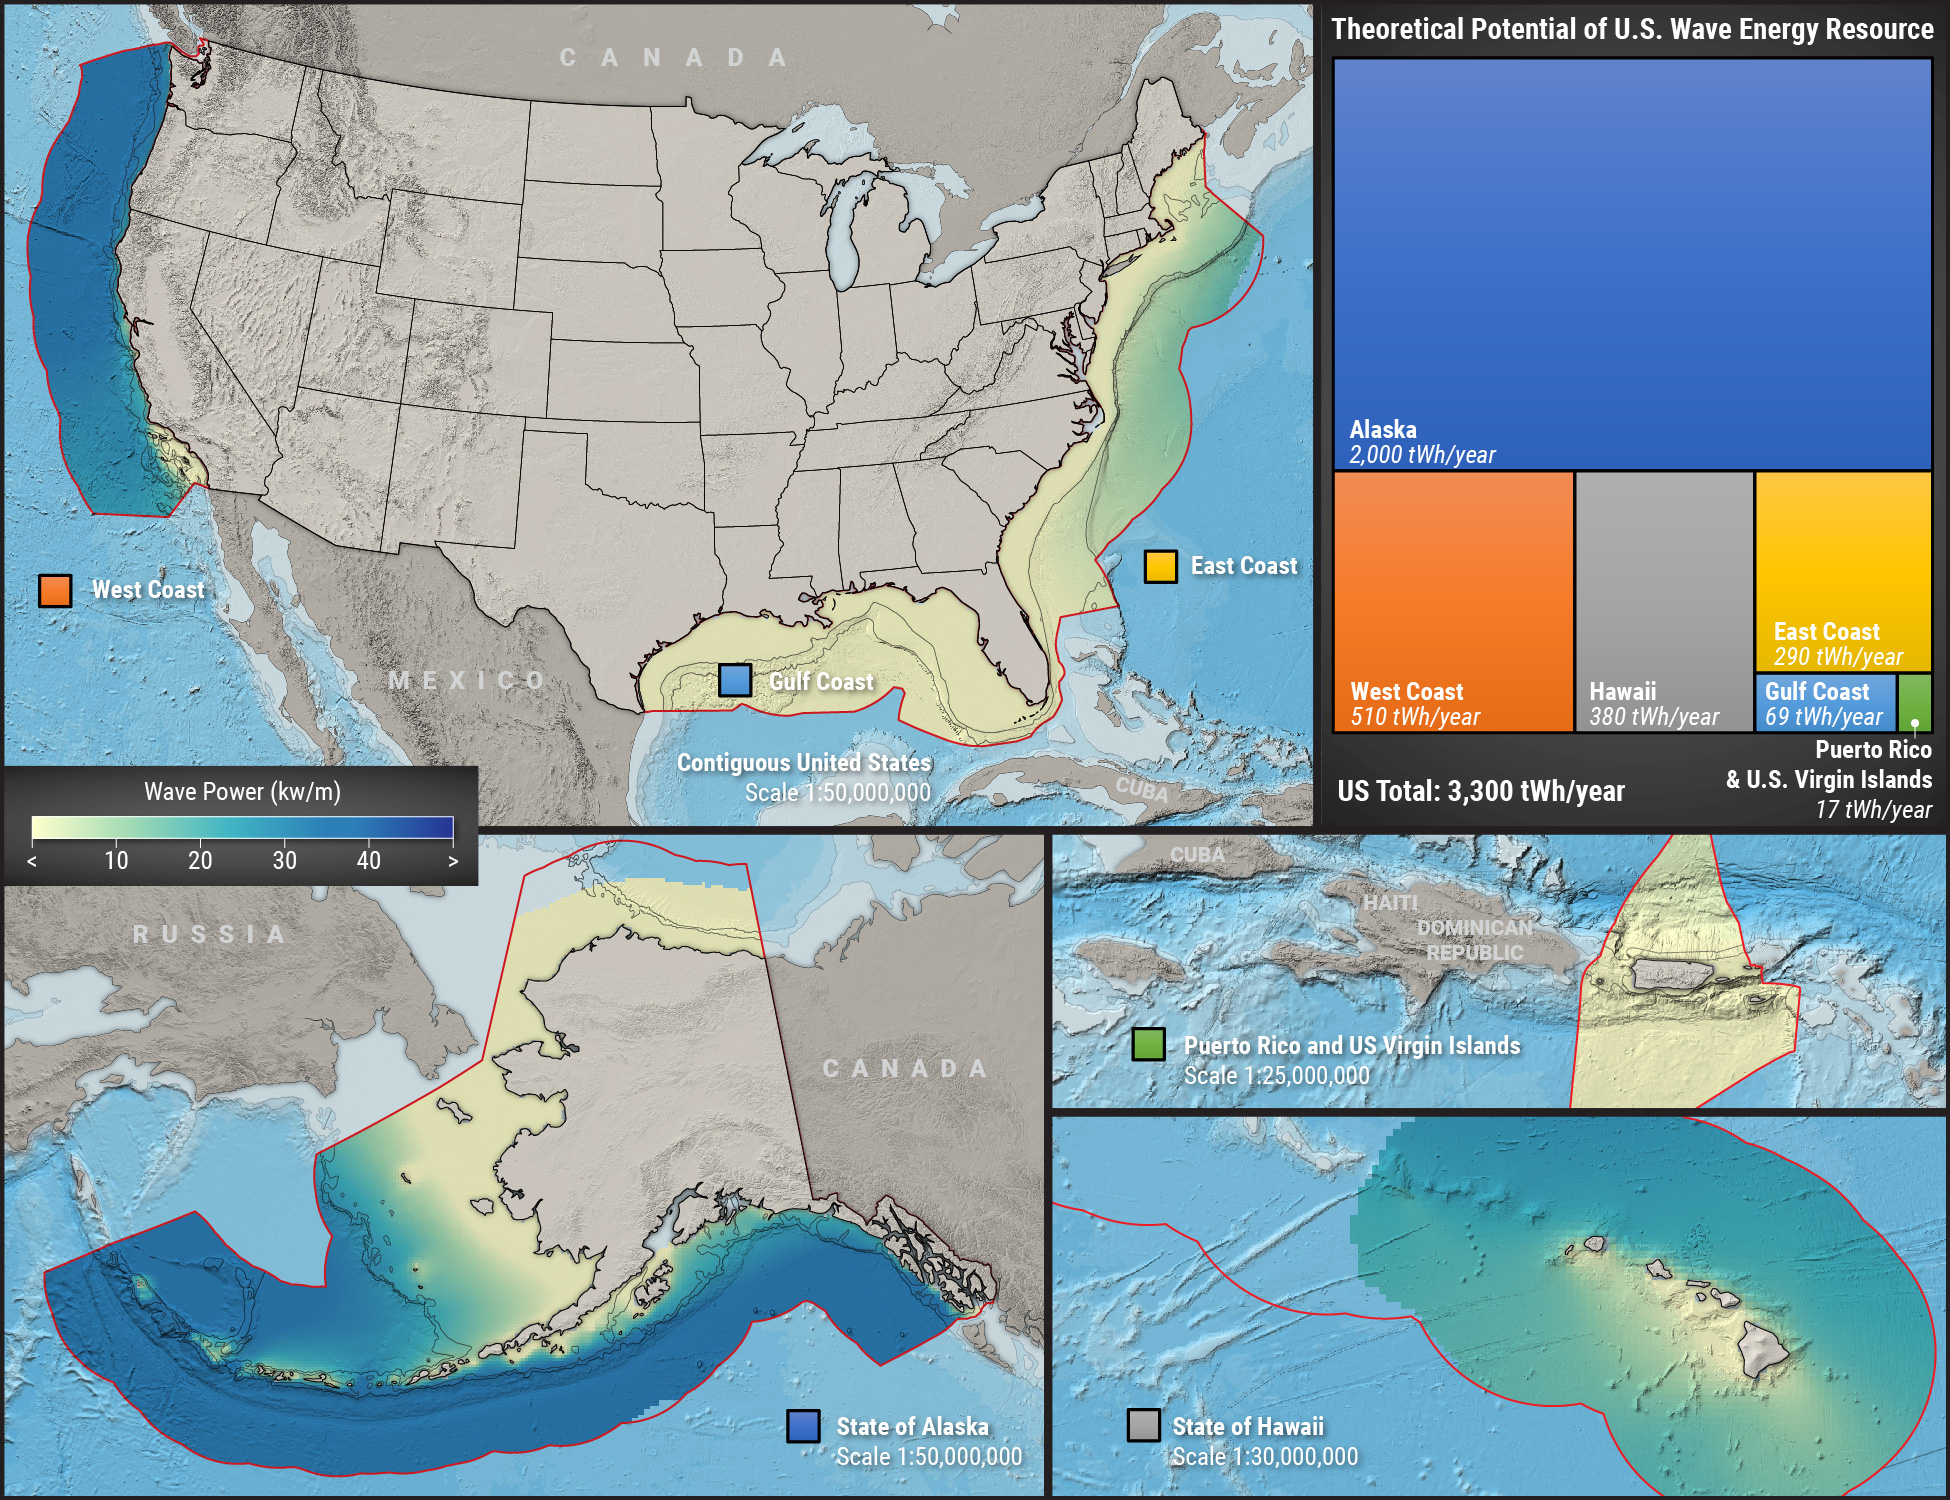
\includegraphics[width=\textwidth]{./fig/Total_Resource_Graphic.png}
  \caption{The U.S. wave energy resource. Maps show the resource intensity (time-average omni-directional wave power) shaded as an ivory to blue (low to high) colormap. The box-diagram in the upper left indicates total resource magnitude by region.}
  \label{fig:map-total}
\end{figure}

%\begin{figure}[ht]
%  \centering
%  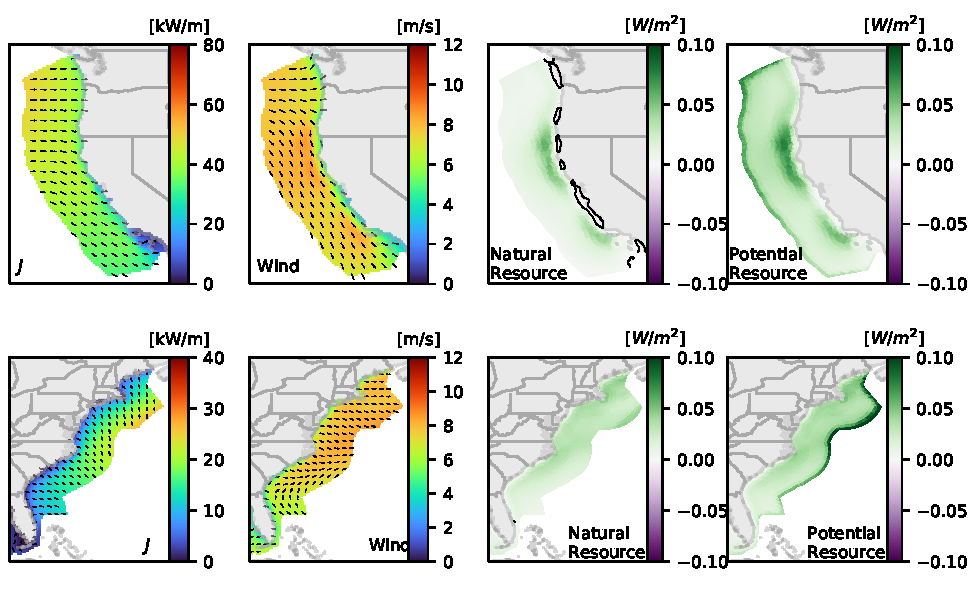
\includegraphics[width=\textwidth]{../fig/Yearly_spatial_seasonal_mag_6.pdf}
%  \caption{Maps of average omnidirectional wave power (left), wind (second column), natural resource (third column), and potential resource (roth) for the West Coast (top) and Atlantic Coast (bottom). Black contours show areas of 0 $W/m^{2}$ local or potential resource.}
%  \label{fig:maps}
%\end{figure}

% \begin{figure}[ht]
%   \centering
%   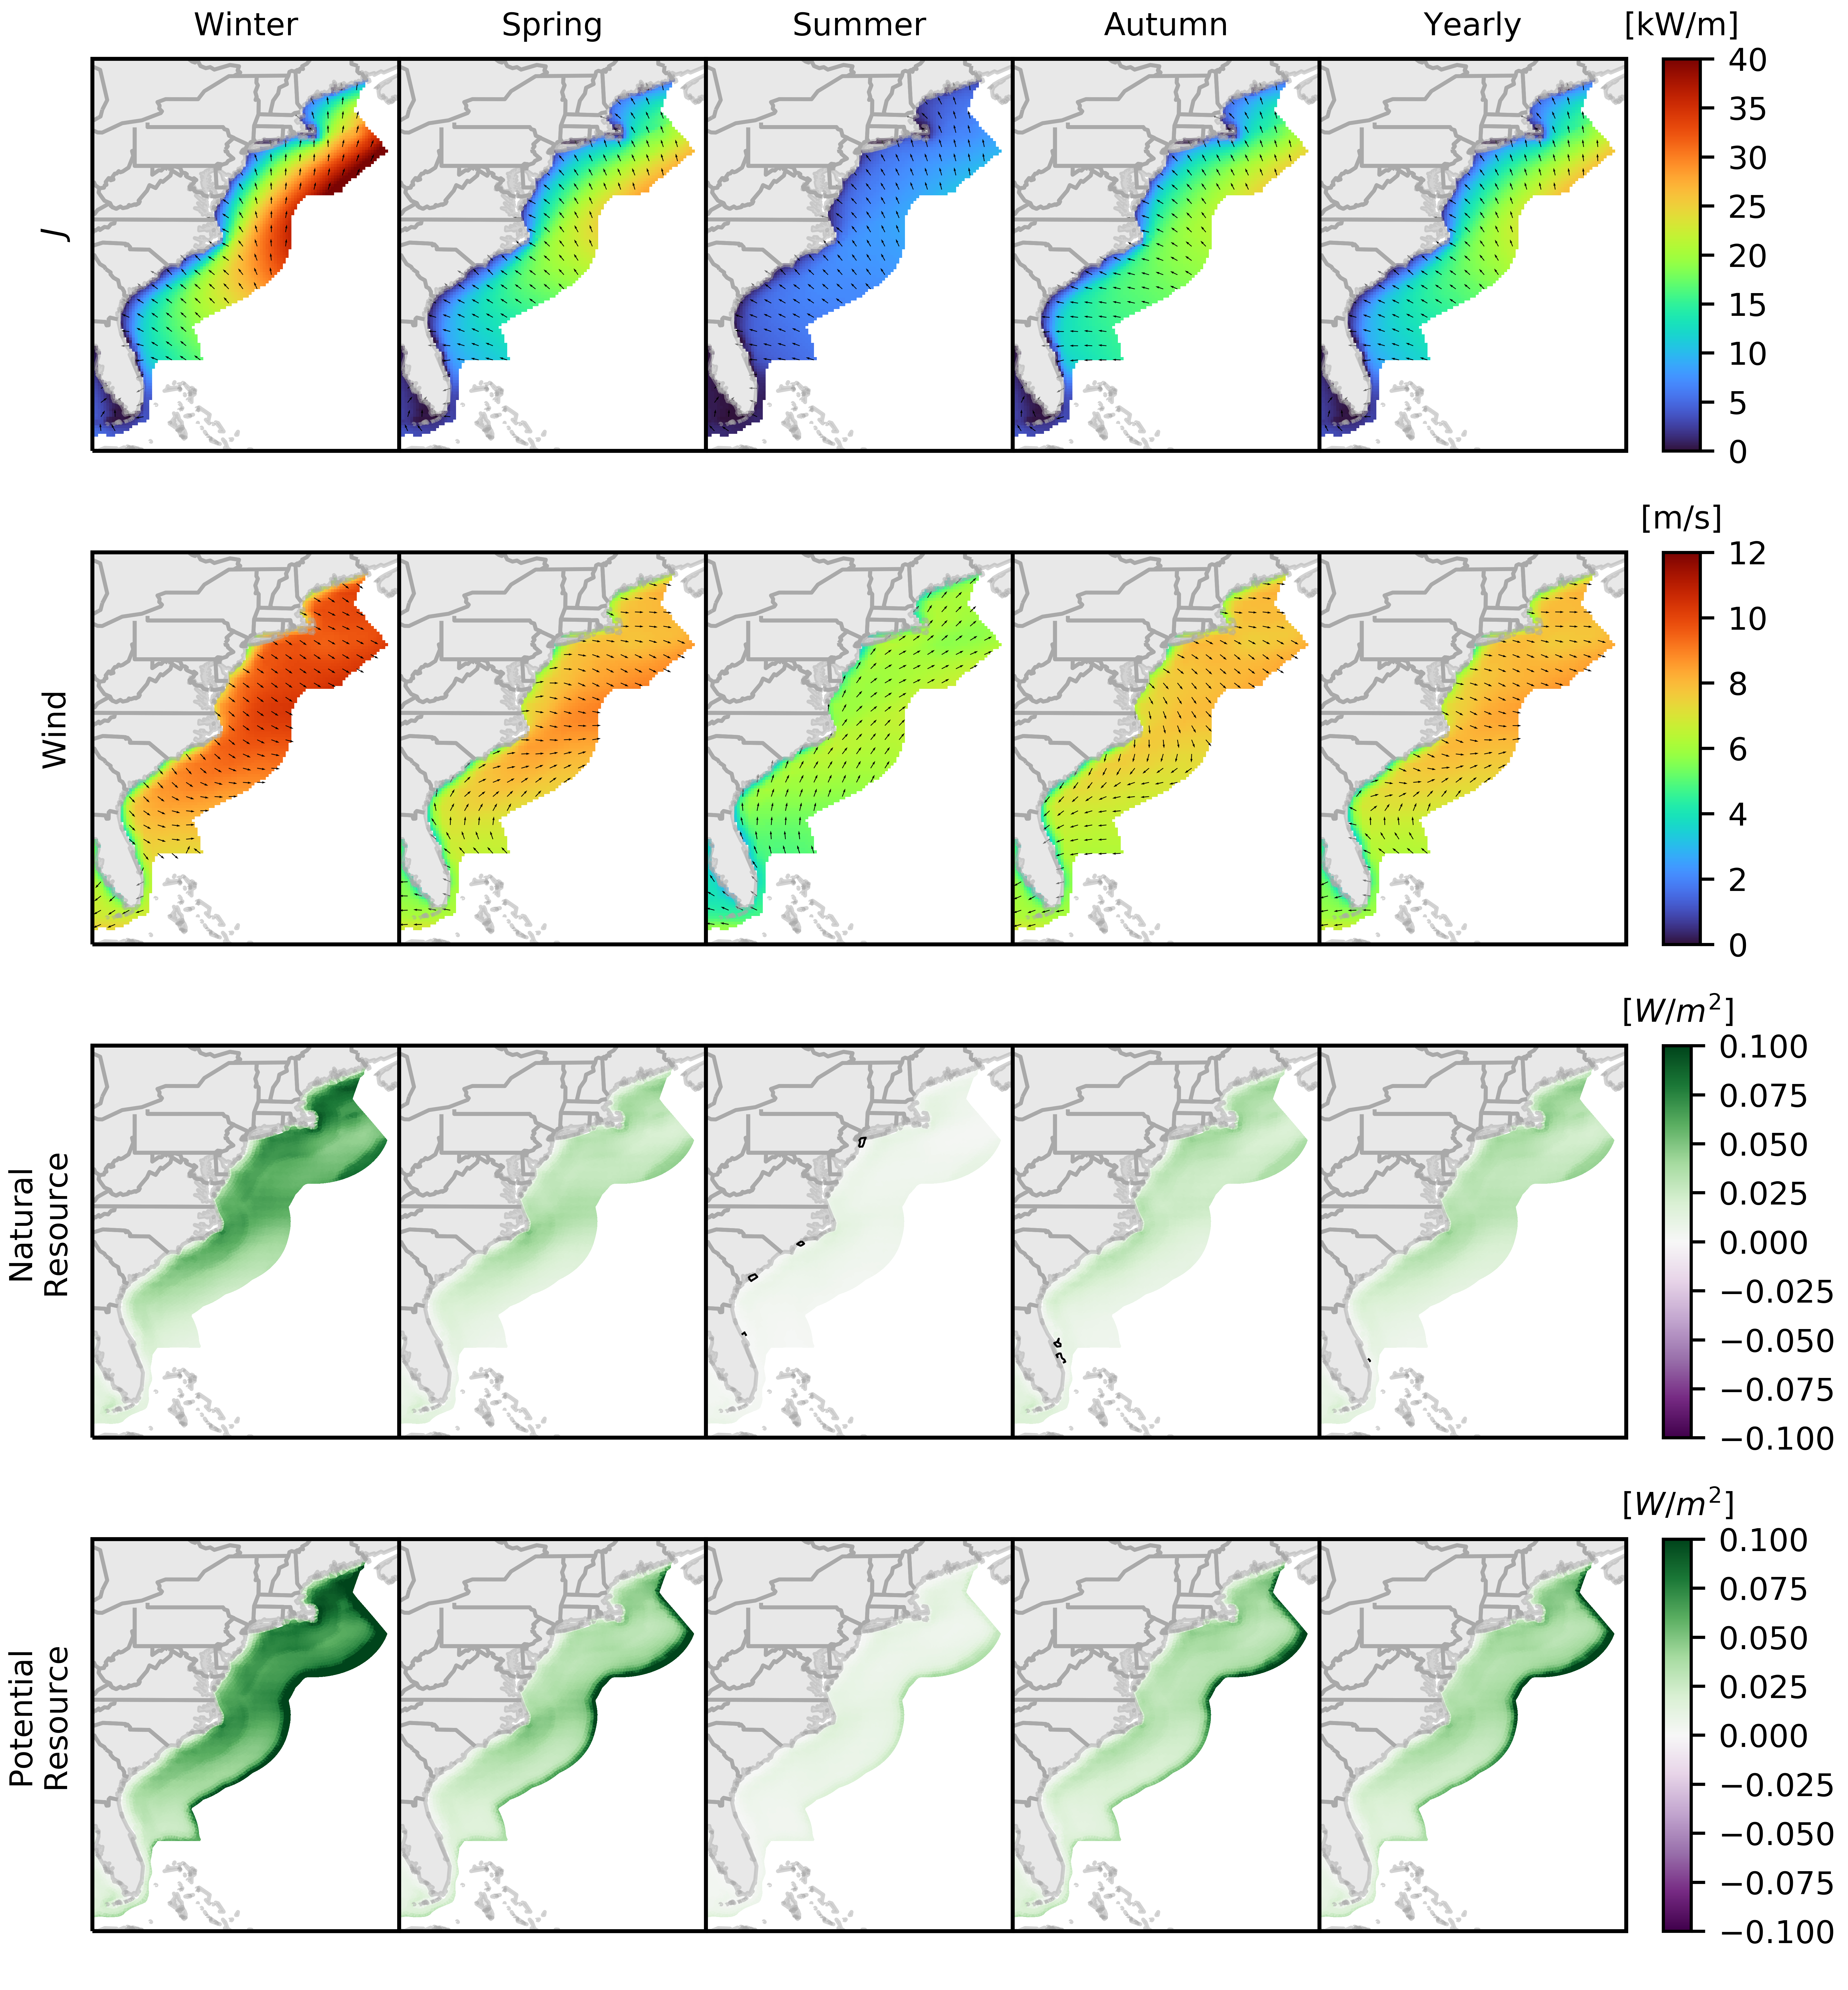
\includegraphics[width=\textwidth]{../fig/at_spatial_seasonal_mag_4.pdf}
%   \caption{Same as \ref{fig:maps-at} for East Coast.}
%   \label{fig:maps-at}
% \end{figure}

\begin{figure}[ht]
  \centering
  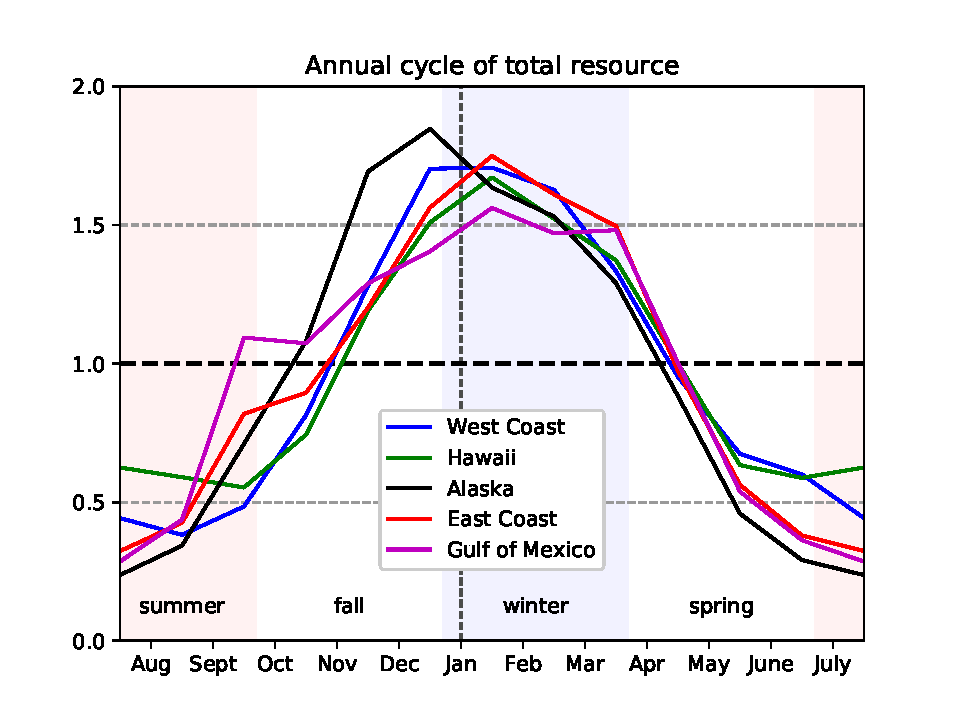
\includegraphics[width=\textwidth]{./fig/AnnualCycle01.pdf}
  \caption[Wave resource annual cycle.]{The annual cycle of the total wave energy resource for several regions, relative to each region's mean.}
  \label{fig:annual-cycle}
\end{figure}


%\begin{figure}[ht]
%  \centering
%  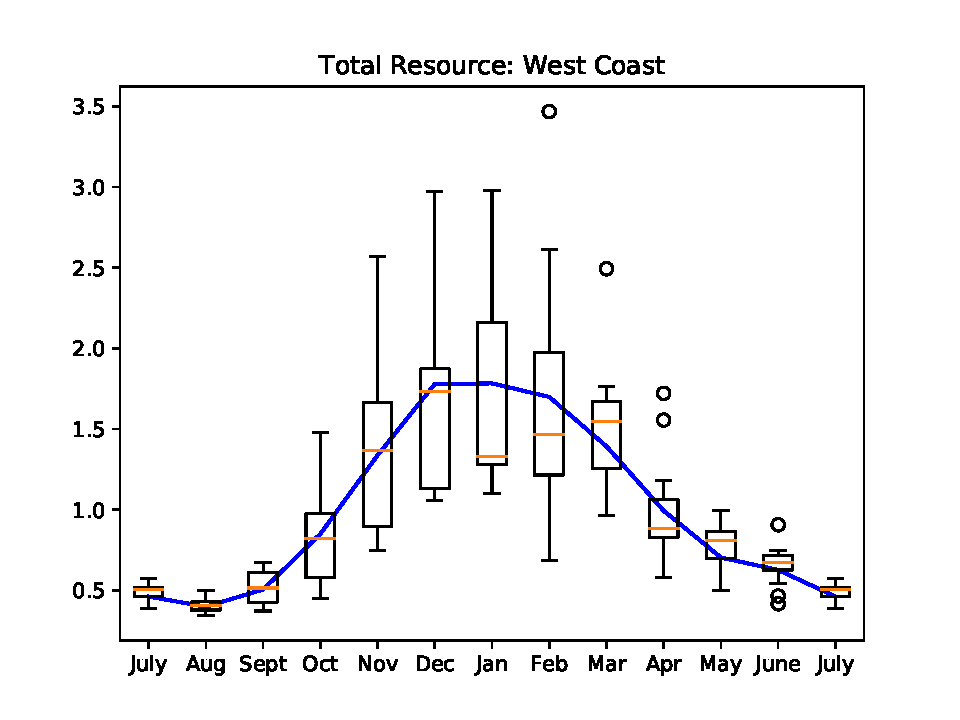
\includegraphics[width=\textwidth]{../fig/AnnualVar01.wc.pdf}
%  \caption[West Coast resource variability.]{Annual and inter-annual variability of the West Coast resource. The thick solid line indicates the mean, and the orange lines and boxes indicate the median and quartiles, respectively. The whiskers extend to the last point within 1.5x of the inter-quartile range, and points beyond this are plotted as open-circles.}
%  \label{fig:wc-variability}
%\end{figure}

\begin{figure}[ht]
  \centering
  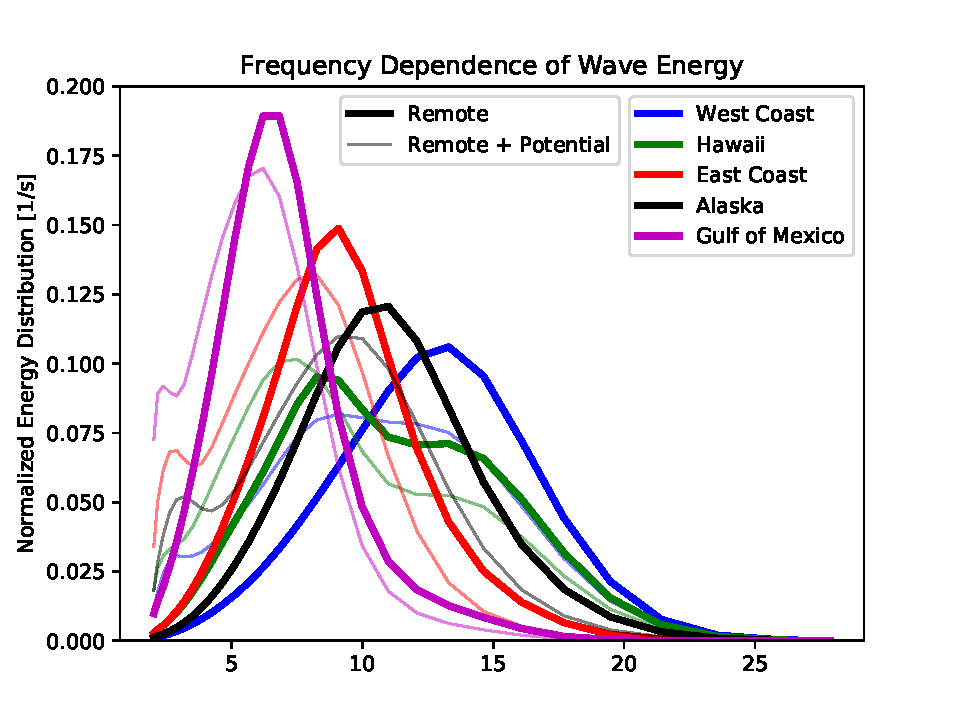
\includegraphics[width=\linewidth]{./fig/TotalResource_Freq02.pdf}
  \caption[Distribution of wave energy vs. wave-period.]{Distribution of wave resource by wave period for each region. Each line represents a spatial average over the entire regional domain. Thick lines indicate the remote resource only, thin lines indicate the sum of the potential and remote resource. Colors are used for each region. Each curve is normalized by its total energy (i.e., the integral of each curve is 1).}
  \label{fig:remote-freq}
\end{figure}

%%% Local Variables:
%%% TeX-master: "wave_res"
%%% End:
